%!TEX root =../mapp-challenge-18-game-book.tex
% ^ leave for LaTeXTools build functionality

\phChapterWorksheet{Wacky Warehouse \mappMobimon{}}{Main Puzzle 1}

While training your \mappMobimon{} on Interstate \( \pi \), you are approached
by
Dockworker Dave, who challenges you to a \mappMobimon{} battle! You of course
accept, because turning him down would be \textbf{rude}.

It was a close match, but you won! Before he gives you your victory money, he
tells you about the \textbf{vermin \mappMobimon{} Tattarat} which infest the
warehouse he works in. He says if you can figure out how the Tattarats
\textbf{hide in the warehouse boxes}, you should be able to catch one of your
very own!

The boxes in the warehouse are always \textbf{stacked and numbered} in a certain
way. Boxes are always pressed up against the \textbf{left wall} of the
warehouse. The boxes have numbers painted on them according to \textbf{two
  simple rules}.
\begin{enumerate}
\item \textbf{No} numbers are ever \textbf{reused} within a single pile of boxes.
\item A pile of boxes has \textbf{standard numbering} if the numbers increase
  horizontally going towards the right \textbf{and} the numbers also increase
  vertically going up.
\end{enumerate}

So \textbf{this pile}
\begin{center}
  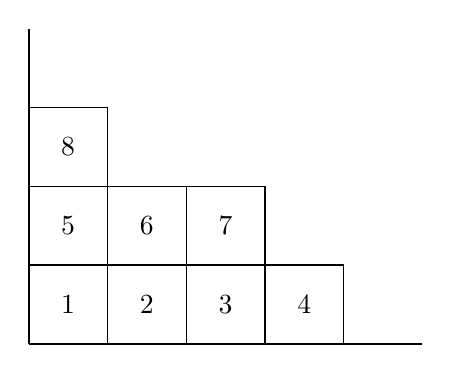
\begin{tikzpicture}
    \draw[thick] (0,0) -- (0, 4);
    \draw[thick] (0,0) -- (5, 0);

    \draw (0,0) grid (1,3);
    \draw (1,0) grid (2,2);
    \draw (2,0) grid (3,2);
    \draw (3,0) grid (4,1);

    \node at (0.5, 0.5){1};
    \node at (1.5, 0.5){2};
    \node at (2.5, 0.5){3};
    \node at (3.5, 0.5){4};

    \node at (0.5, 1.5){5};
    \node at (1.5, 1.5){6};
    \node at (2.5, 1.5){7};

    \node at (0.5, 2.5){8};
  \end{tikzpicture}
\end{center}
is \textbf{standard}.

However \textbf{this pile}
\begin{center}
  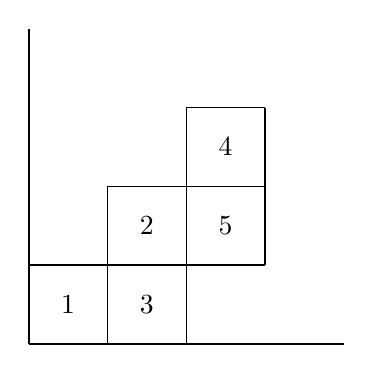
\begin{tikzpicture}
    \draw[thick] (0,0) -- (0,4);
    \draw[thick] (0,0) -- (4,0);

    \draw (0,0) grid (1,1);
    \draw (1,0) grid (2,2);
    \draw (2,1) grid (3,3);

    \node at (0.5, 0.5){1};
    \node at (1.5, 0.5){3};
    \node at (1.5, 1.5){2};

    \node at (2.5, 1.5){5};
    \node at (2.5, 2.5){4};
  \end{tikzpicture}
\end{center}

is \textbf{not} standard, for three different reasons.
\begin{itemize}
\item The boxes aren't all pushed to left wall!
\item The boxes aren't numbered in increasing order from bottom to top!
\item Wait, boxes 4 and 5 are floating above the floor! How does that even work?
  That's not right.
\end{itemize}



%%% Local Variables:
%%% mode: latex
%%% TeX-master: "../mapp-challenge-18-game-book"
%%% End:
